\documentclass[professionalfonts,compress,unicode]{beamer}

\usepackage{amsmath,amssymb}
\usepackage[utf8]{inputenc}

\usepackage[russian]{babel}

\usepackage{multirow}
\usepackage{colortbl}

\usetheme{Warsaw}
\usecolortheme{uranix}

\setbeamertemplate{headline}
{%
  \begin{beamercolorbox}[sep=0.3cm,wd=\paperwidth]{section in head/foot}%
    \usebeamerfont{frametitle}%
    \vbox{}\vskip-1ex%
    \strut\insertsectionhead\strut\par%
    \vskip-1ex%
  \end{beamercolorbox}%
}
\setbeamertemplate{navigation symbols}{}
\setbeamertemplate{footline}{}

\renewcommand{\thefootnote}{\fnsymbol{footnote}}

\graphicspath{{images//}}

\title[Интегрирование]{Численное интегрирование}
\author[Цыбулин И.В.]{Скалько Юрий Иванович\\
\textbf{Цыбулин Иван}
}
\date{}
%\vspace{0.3cm}

\begin{document}

{
\setbeamertemplate{headline}[default]
\frame{
\titlepage
}

%\frame{
%\frametitle{Содержание}
%\small
%%\tiny
%\tableofcontents
%}
}

\newcommand\myframe[2]{\subsection{#1}\frame{\frametitle{#1}{#2}}}

\section{ }

\section{Интегрирование}
\myframe{Задача численного интегрирования}
{
	\begin{block}{Задача}
		Задана функция $f(x)$. Вычислить $\int_a^b f(x) dx$.
	\end{block}
	\pause
	
	Вначале рассмотрим случай собственного интеграла, то есть 
	\begin{itemize}
		\item $a$ и $b$ --- действительные числа (не $\pm \infty$)
		\item $f(x)$ не имеет на $[a,b]$ особых точек
	\end{itemize}
	\pause
	
	Интеграл можно определить как предел интегральных сумм
	$$
	\int_a^b f(x) dx = \lim_{\max \Delta x_i \rightarrow 0} \sum_{i=1}^{n-1} f(\xi_i) \Delta x_i,\quad \xi_i \in [x_i,x_{i+1}]
	$$
}

\myframe{Простейший численный метод}
{
	$$
	\int_a^b f(x) dx = \lim_{\max \Delta x_i \rightarrow 0} \sum_{i=1}^{n-1} f(\xi_i) \Delta x_i,\quad \xi_i \in [x_i,x_{i+1}]
	$$
	
	Введем на отрезке некоторую сетку $\left\{x_i\right\}_{i = 1}^n$. В качестве $\xi_i$ возьмем, например, середину $i$-го отрезка
	$ \xi_i = \frac{x_i+x_{i+1}}{2} $
	\pause
	$$
	\int_a^b f(x) dx \approx \sum_{i=1}^{n-1} f\left(\frac{x_i+x_{i+1}}{2}\right)\Delta x_i
	$$
	\pause
	
	Полученный метод называется \emph{формулой прямоугольников} или \emph {формулой средней точки}. 
	Формулы численного интегрирования также называют \emph{квадратурными формулами}
}

\myframe{Формула прямоугольников}
{
	\begin{figure}%
	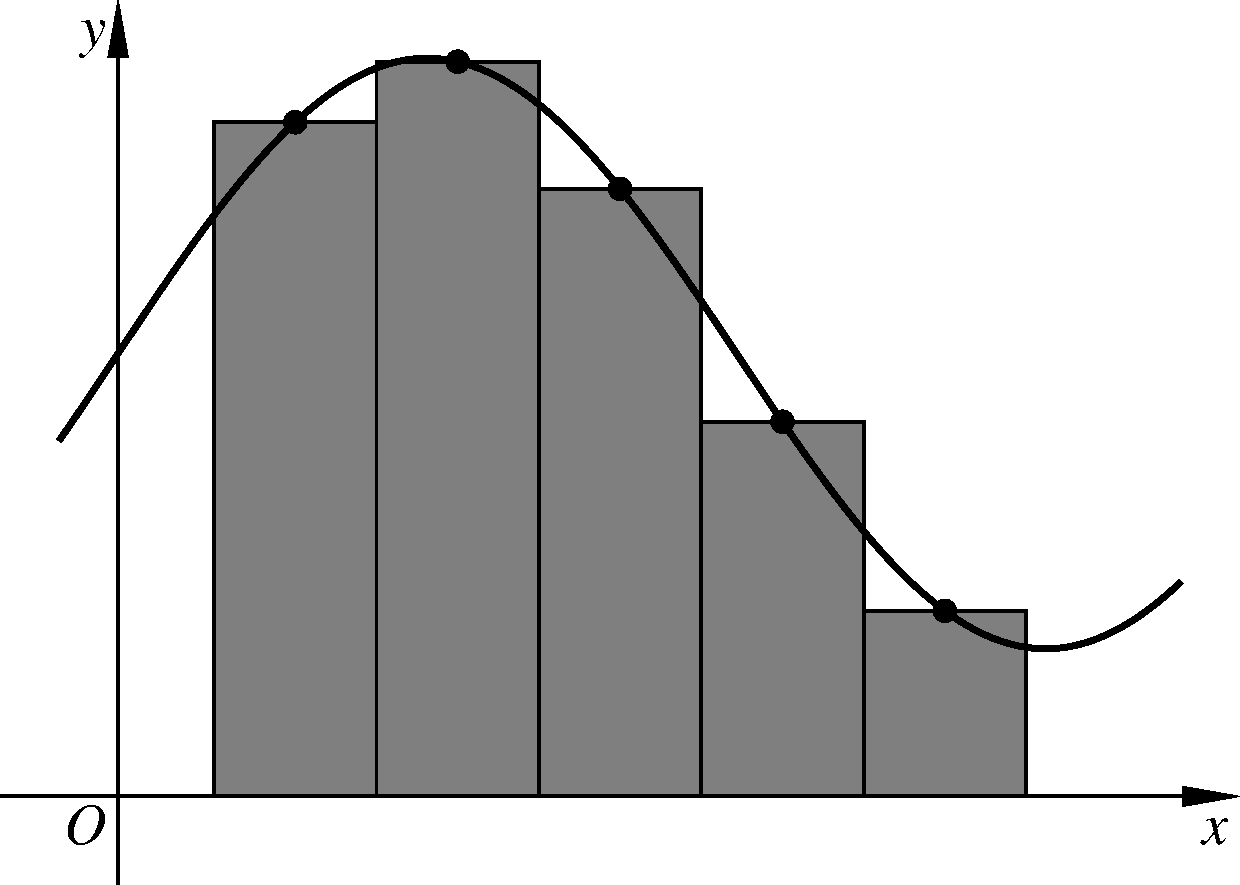
\includegraphics[width=\columnwidth]{rect.pdf}%
	\end{figure}
}

\myframe{Формула односторонних прямоугольников}
{
	Ничего не запрещает в формуле прямоугольников вместо средней точки брать крайнюю, например левую.
	Интуитивно такой выбор хуже, но к этому вернемся позднее.
	$$
	\int_a^b f(x) dx \approx \sum_{i=1}^{n-1} f\left(x_i\right)\Delta x_i
	$$
	$$
	\int_a^b f(x) dx \approx \sum_{i=1}^{n-1} f\left(x_{i+1}\right)\Delta x_i
	$$
	
	\pause
	
	Такие формулы называются формулами \emph{левых} и \emph{правых прямоугольников}
}

\myframe{Формулы левых и правых прямоугольников}
{
	\begin{figure}%
	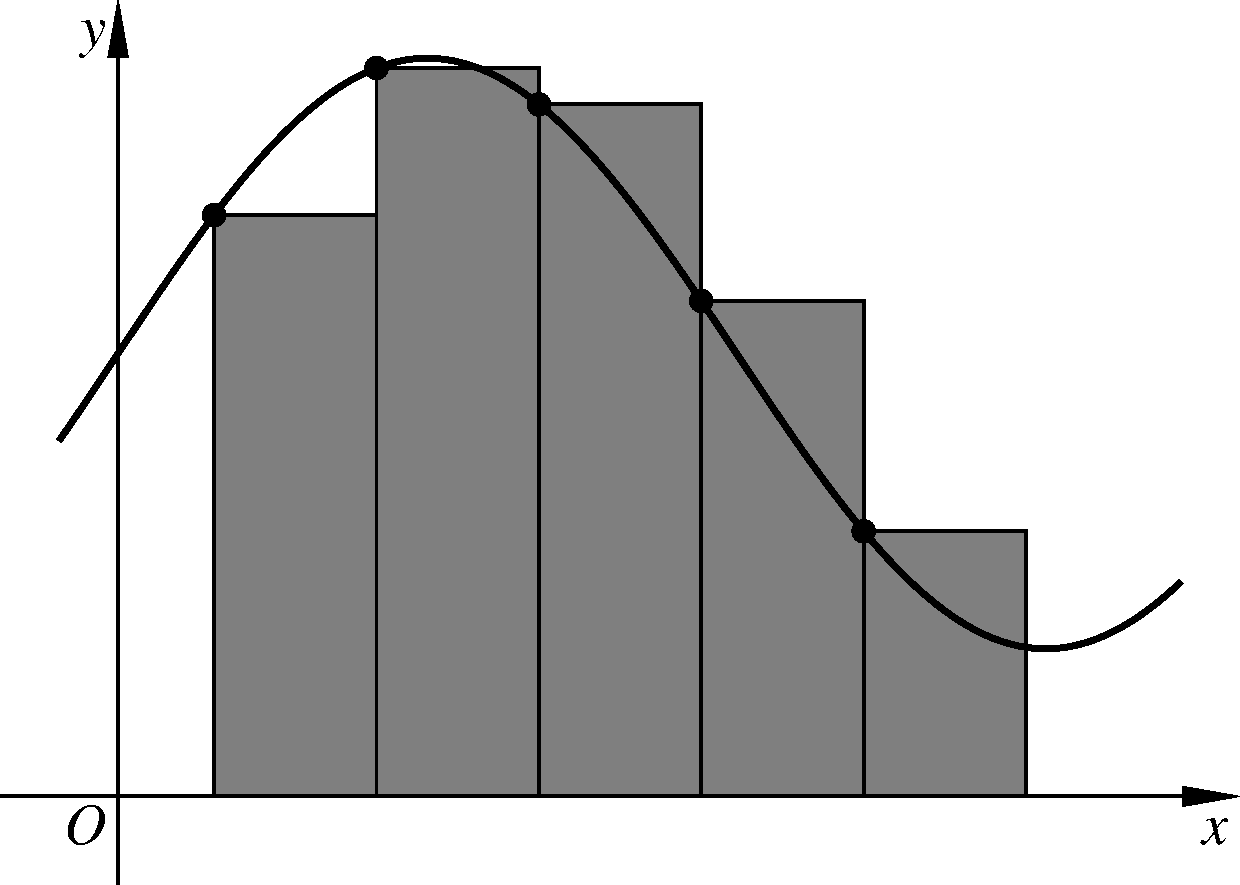
\includegraphics[width=.5\columnwidth]{lrect.pdf}%
	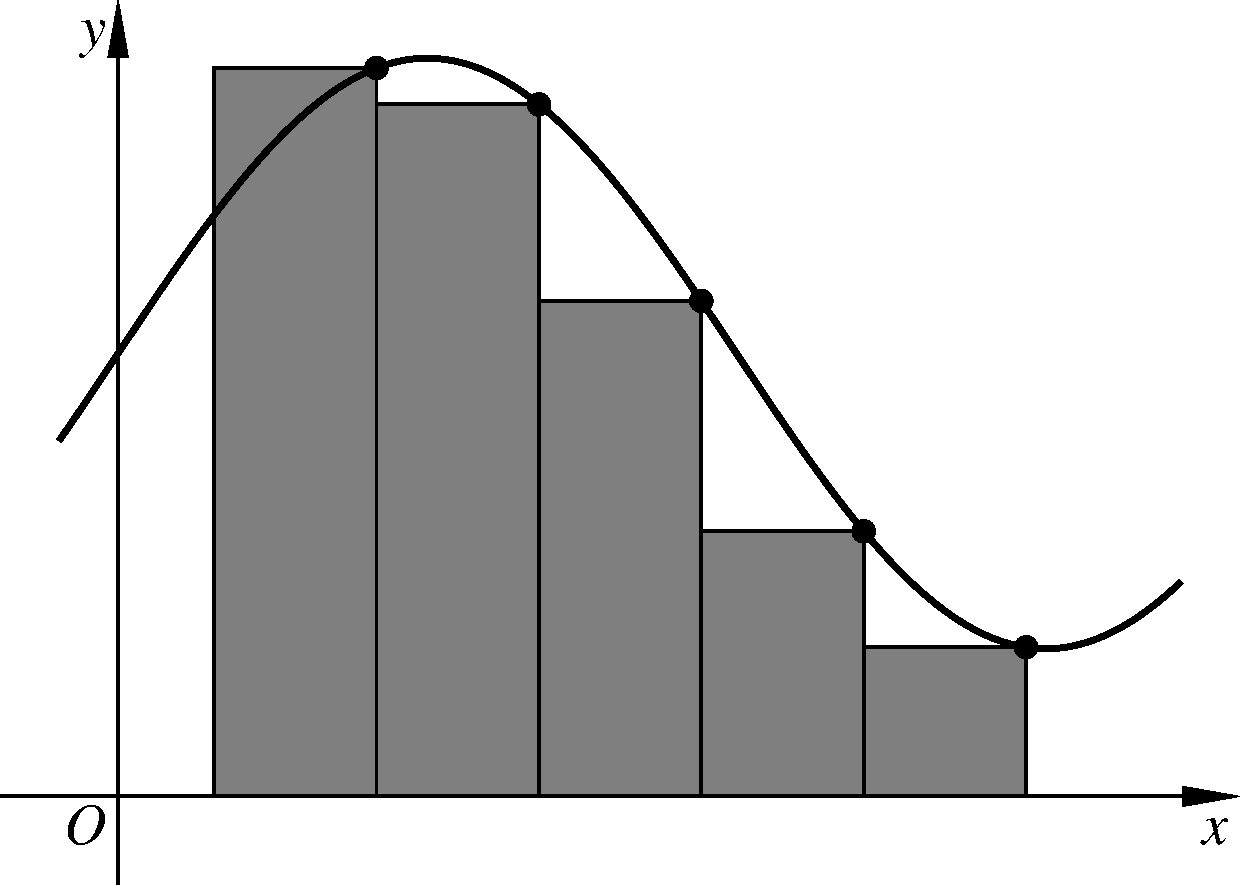
\includegraphics[width=.5\columnwidth]{rrect.pdf}%
	\end{figure}
}

\myframe{Более точные формулы}
{
	Заменим функцию $f(x)$ некоторой более простой функцией $g(x)$, которая легко 
	интегрируется.
	\pause
	
	Проще всего взять в качестве функции $g(x)$ многочлен. Тогда задача приближения 
	функции $f(x)$ многочленом легко решается с помощью интерполяции. 
	\pause
	
	Приближать функцию $f(x)$ многочленом высокой степени нежелательно, 
	вследствие возможного роста ошибки интерполяции при большом числе узлов. 
	Можно воспользоваться простейшим сплайном (для приближения гладкость $g(x)$ не важна) ---
	кусочно многочленной интерполяцией.
}

\myframe{Более точные формулы}
{
	По-аналогии с формулой прямоугольников, введем на отрезке интегрирования сетку, но теперь на каждом
	интервале приблизим функцию не константой, как в методе средней точки $f(x) \approx f\left(\frac{x_i+x_{i+1}}{2}\right)$,
	а многочленом степени $p$: $f(x) \approx Q_i(x)$.
	$$
	\int_a^b f(x) dx\approx \sum_{i=1}^{n-1} \int_{x_i}^{x_{i+1}} Q_i(x) dx
	$$
}

\myframe{$p=1$. Формула трапеций}
{
	Рассмотрим случай линейных функций $Q_i(x)$. 
	$$
	Q_i(x) = 
	%f(x_i)+\frac{f(x_{i+1})-f(x_i)}{x_{i+1}-x_i} (x-x_i) = 
	\frac{x_{i+1}-x}{x_{i+1}-x_i} f(x_i) + \frac{x-x_i}{x_{i+1}-x_i} f(x_{i+1})
	$$
	\pause
	Проинтегрировав (представление в форме Лагранжа удобнее интегрировать), получаем
	$$
	\int_{x_i}^{x_{i+1}} Q_i(x) dx = \frac{x_{i+1}-x_i}{2} f(x_i) + \frac{x_{i+1}-x_i}{2} f(x_{i+1})
	$$
	$$
	\int_a^b f(x) dx \approx \sum_{i=0}^{n-1} \frac{f(x_i)+f(x_{i+1})}{2} \Delta x_i
	$$
	Полученная формула называется \emph{формулой трапеций}.
}

\myframe{Формула трапеций}
{
	\begin{figure}%
	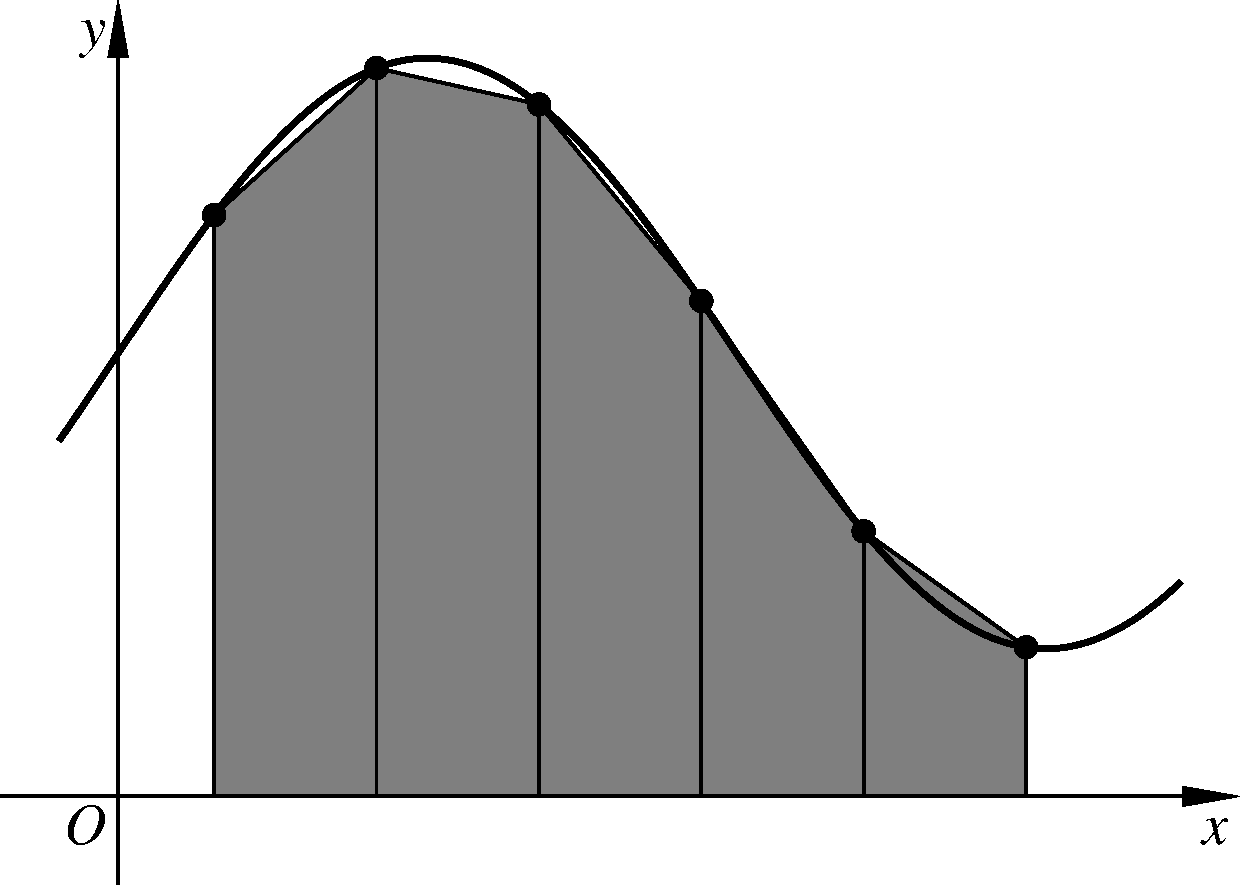
\includegraphics[width=\columnwidth]{trap.pdf}%
	\end{figure}
}

\myframe{Интерполяционные формулы}
{
	При построении формулы трапеций представление $Q_i(x)$ в виде Лагранжа оказалось
	весьма удобным. Покажем, как обобщить эту формулу на произвольный порядок $p$.
	\pause
	
	Введем теперь на каждом отрезке $[x_i, x_{i+1}]$ свою внутреннюю сетку из $p$ узлов: 
	$$\left\{x_i^s\right\}_{s=1}^p,\quad x_i = x_i^1,\quad x_{i+1}=x_i^p$$
	\pause
	
	Тогда для $Q_i(x)$ справедливо представление
	$$
	Q_i(x) = \sum_{s=1}^p \ell_s(x) f(x_i^s)
	$$
	$$
	\int_{x_i}^{x_{i+1}} Q_i(x) dx = \sum_{s=1}^p f(x_i^s) \int_{x_i}^{x_{i+1}} \ell_s(x) dx
	$$	
}

\myframe{Интерполяционные формулы}
{
	Интегрирование функции $Q_i(x)$ свелось к интегрированию базисных многочленов Лагранжа.
	$$
	\int_{x_i}^{x_{i+1}} Q_i(x) dx = \sum_{s=1}^p f(x_i^s) \int_{x_i}^{x_{i+1}} \ell_s(x) dx
	$$
	\pause
	Если дополнительно предположить, что на каждом отрезке внутренние сетки отличаются только масштабом 
	(например, всюду равномерные или всюду чебышевские), 
	то интегралы от $\ell_s(x)$ будут отличаться только множителем $\Delta x_i$
	$$
	\int_{x_i}^{x_{i+1}} \ell_s(x) dx \equiv \gamma_s \Delta x_i
	$$
	\pause
	Квадратурная формула записывается в виде
	$$
	\int_a^b f(x) dx \approx \sum_{i=1}^{n-1} \left(\sum_{s=1}^p \gamma_s f(x_i^s)\right)\Delta x_i
	$$
}

\myframe{$p=2$. Формула Симпсона}
{
	В этом случае на каждом отрезке функция приближается параболой. Для этого требуются значения в трех точках ---
	в концах отрезка и в центре. Вычисляя коэффициенты $\gamma_s$ 
	$$
	\gamma_1 = \frac{1}{6}, \quad \gamma_2 = \frac{2}{3}, \quad \gamma_3 = \frac{1}{6}
	$$
	и подставляя в общую формулу, получаем \emph{формулу Симпсона}
	$$
	\int_a^b f(x) dx \approx \sum_{i=1}^{n-1} \frac{f(x_i) + 4f\left(\frac{x_i+x_{i+1}}{2}\right) + f(x_{i+1})}{6} \Delta x_i
	$$
	Хотя данная формула точнее формулы трапеций и средней точки, она требует в два раза больше вычислений функции $f(x)$.
	
%	В случае когда сетка $\left\{x_i\right\}_{i=1}^n$ равномерная, можно пользоваться четными точками как серединами отрезков
%	вдвое большей длины $[x_{2k-1},x_{2k+1}]$. 
}

\myframe{Что точнее?}
{
	\begin{figure}%
	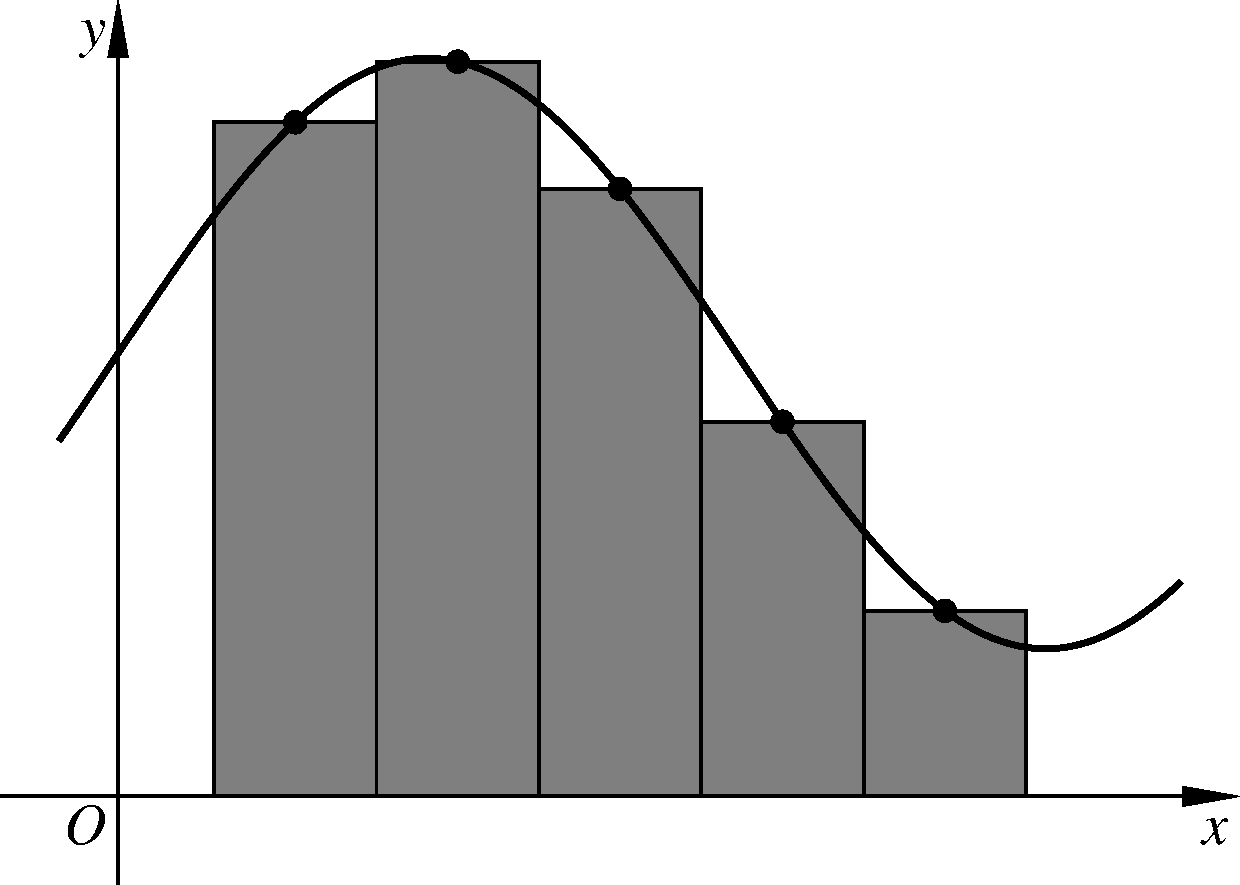
\includegraphics[width=0.5\columnwidth]{rect.pdf}%
	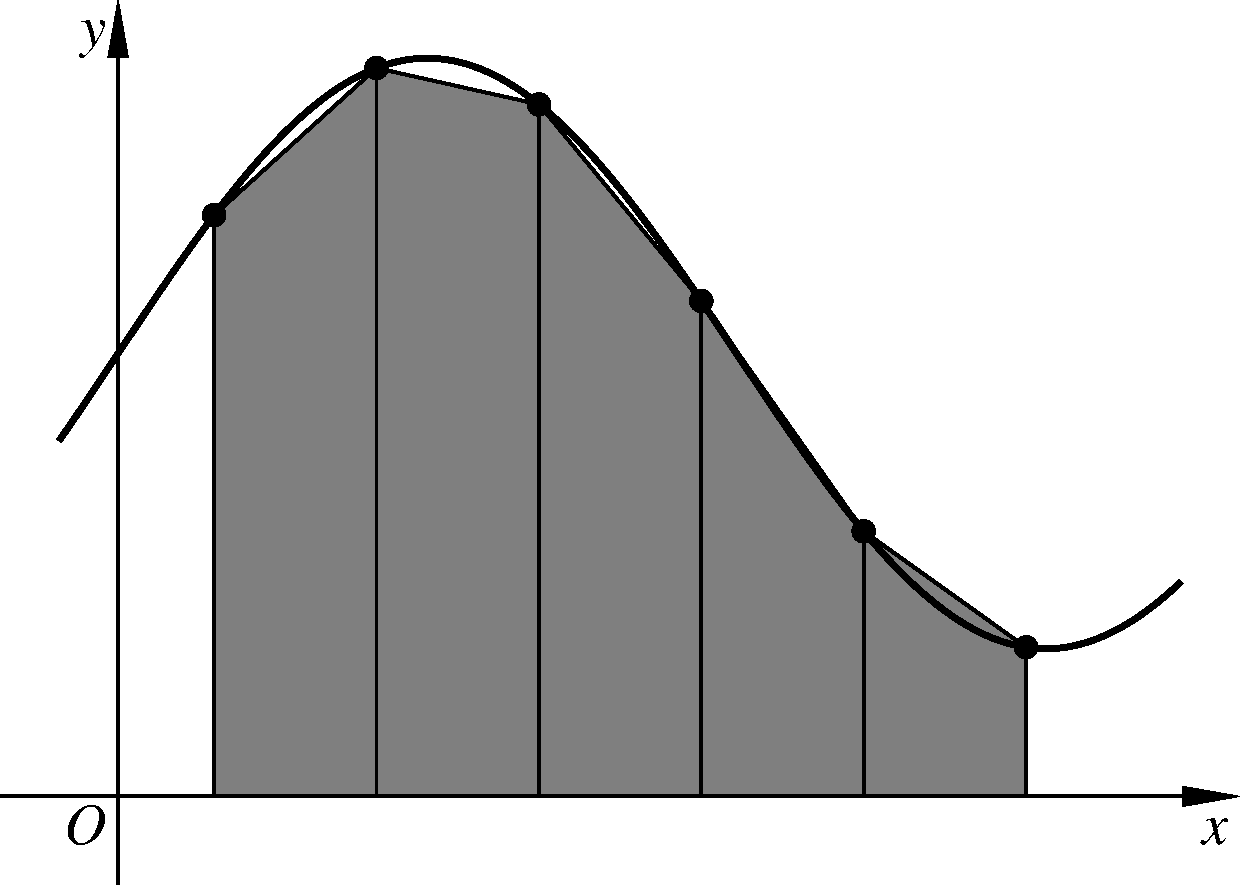
\includegraphics[width=0.5\columnwidth]{trap.pdf}%
	\end{figure}
	\pause
	
	\begin{columns}[c]
	\begin{column}{0.5\textwidth}
	\centering
	Ошибка $\approx 1\%$
	\end{column}
	\begin{column}{0.5\textwidth}
	\centering
	Ошибка $\approx 2\%$
	\end{column}
	\end{columns}
}

\myframe{Ошибка интерполяции}
{
	Ошибка интерполяции, то есть отличие точного значения интеграла от вычисленного, в худшем случае,
	просуммируется по всем интервалам сетки. Поэтому, найдем ошибку интегрирования функции только на одном отрезке.
	Для простоты, обозначим его $[a,b], \, h = b-a$.
	$$
	\int_a^b f(x) dx \approx h \sum_{s=1}^p \gamma_s f(x_s) 
	$$
	\pause
	Поскольку интегрирование --- это линейная операция,
	квадратурные формулы также линейны по значениям функции $f(x)$. Здесь $\gamma_s$ --- просто некоторые 
	коэффициенты квадратурной формулы.
}

\myframe{Ошибка интерполяции}
{
	$$
	\int_a^b f(x) dx \approx h \sum_{s=1}^p \gamma_s f(x_s) 
	$$
	Возьмем некоторую точку $z$. Конкретное значение несущественно, но удачный выбор точки $z$ может сильно сократить объем 
	вычислений. \pause Представим функцию $f(x)$ в виде формулы Тейлора в окрестности точки $z$
	$$
	f(x) = f(z) + (x-z)f'(z) + \frac{(x-z)^2}{2}f''(z) + \dots + \frac{(x-z)^{m}}{m!}f^{(m)}(\zeta(x))
	$$
	Если формулу Тейлора проинтегрировать
	$$
	\int_a^b f(x) dx = h f(z) + \left.\frac{(x-z)^2}{2}\right|_a^b f'(z) + \dots + \int_a^b \frac{(x-z)^{m}}{m!}f^{(m)}(\zeta(x)) dx
	$$
}

\myframe{Ошибка интерполяции}
{
	$$
	\int_a^b f(x) dx = h f(z) + \left.\frac{(x-z)^2}{2}\right|_a^b f'(z) + \dots + \int_a^b \frac{(x-z)^{m}}{m!}f^{(m)}(\zeta(x)) dx
	$$
	Разложим аналогично правую часть
	\begin{align*}
	%\int_a^b f(x) dx \approx 
		h \sum_{s=1}^p \gamma_s f(x_s) = h \sum_{s=1}^p &\gamma_s f(z) + h \sum_{s=1}^p (x_s-z)\gamma_p f'(z) + \\
	\dots&+ h \sum_{s=1}^p \gamma_s \frac{(x-z)^{m}}{m!} f^{(m)}(\zeta(x_s))
	\end{align*}
	Ошибка интегрирования получается из разности первых не совпадающих выражений перед одинаковыми производными. В частности, для всех 
	квадратурных формул должно быть $\sum_{s=1}^p \gamma_s = 1$, а для формул выше первого порядка $\sum_{s=1}^p \gamma_s x_s = \frac{a+b}{2}$.
}

\myframe{Ошибка интерполяции}
{
	Анализируя представления в виде формулы Тейлора, можно заключить, что
	ошибка интерполяции квадратурных формул имеет вид (для одного отрезка)
	$$
	\varepsilon_{\text{метода}} \leq C h^{r+1} M_r,
	$$
	где $C$ - некоторая числовая константа.
	Суммируя ошибку по всем отрезкам
	$$
	\varepsilon_{\text{метода}} \leq C \sum_{i=1}^{n-1} h_i^{r+1} M_{r,i} \leq C \max_i \left(M_r h^r\right) \sum_{i=1}^{n-1} h_i = 
	C(b-a)\max_i \left(M_r h^r\right)
	$$
	Здесь хорошо видно, что имеет смысл уменьшать шаг $h_i$ на тех отрезках, где $r$-я производная начинает 
	сильно возрастать по модулю.
}

\myframe{Погрешность метода средней точки}
{
	Рассмотрим один интервал $a=x_i, b=x_{i+1}$.
	Возьмем в качестве опорной именно среднюю точку $z = \frac{a+b}{2}$.
	$$
	f(x) = f(z) + (x-z)f'(z) + \frac{(x-z)^2}{2}f''(\zeta)
	$$
	$$
	\int_a^b f(x) dx = h f(z) + \int \frac{(x-z)^2}{2}f''(\zeta) dx
	$$
	$$
	\varepsilon_{\text{метод}} \leq \left|\int \frac{(x-z)^2}{2}f''(\zeta) dx \right|
	\leq M_2 \int \left|\frac{(x-z)^2}{2}\right| dx  = M_2 \frac{h^3}{24}
	$$
	При этом на всем отрезке справедлива оценка
	$$
	\varepsilon_{\text{метод}} \leq (b-a) \frac{M_2h^2}{24}
	$$
}

\myframe{Погрешность метода трапеций}
{
	Рассмотрим один интервал $a=x_i, b=x_{i+1}$.
	Воспользуемся формулой Тейлора с остаточным членом в форме Пеано. В качестве опорной точки возьмем $z = \frac{a+b}{2}$
	$$
	f(x) = f(z) + (x-z)f'(z) + \frac{(x-z)^2}{2}f''(z) + o((x-z)^2)
	$$
	$$
	\int_a^b f(x) dx = h f(z) + 2\frac{(b-z)^3}{6}f''(z) + o(h^3) = hf(z) + \frac{h^3}{24}f''(z) + o(h^3)
	$$
	$$
	f\left(z \pm \frac{h}{2}\right) = f(z) \pm \frac{h}{2} f'(z) + \frac{h^2}{8} f''(z) + o(h^2)
	$$
	$$
	h\frac{f(a)+f(b)}{2} = hf(z) + \frac{h^3}{8} f''(z) + o(h^3)
	$$
	Вычитая разложение квадратуры из разложения интеграла получаем ошибку
	$$
	\Delta = \frac{h^3}{24}f''(z) - \frac{h^3}{8}f''(z) + o(h^3) = -\frac{h^3}{12}f''(z) + o(h^3).
	$$
}

\myframe{Погрешность метода трапеций}
{
	Мы показали, что в пределах одного отрезка 
	$$
	\int_a^b f(x) dx = h\frac{f(a)+f(b)}{2} - \frac{h^3}{12}f''\left(\frac{a+b}{2}\right) + o(h^3)
	$$
	Оценка через остаточный член в форме Лагранжа дает ошибку в два раза большую
	$$
	\varepsilon_{\text{метод}} \leq \frac{M_2 h^3}{6}
	$$
	Однако, более тонкими рассуждениями можно показать, что
	$$
	\int_a^b f(x) dx = h\frac{f(a)+f(b)}{2} - \frac{h^3}{12}f''(\xi)
	$$
	то есть асимптотическая оценка является точной.  На всем отрезке верна оценка
	$$
	\varepsilon_{\text{метод}} \leq (b-a) \frac{M_2 h^2}{12}
	$$	
}

\myframe{Погрешность метода Симпсона}
{
	Аналогично, для метода Симпсона без дополнительных точек можно получить 
	асимптотическую оценку на интервалах
	$$
	\varepsilon_{\text{метод}} = \frac{f^{IV}(z) h^5}{180} + o(h^5)
	$$
	Эта оценка также допускает строгое обоснование
	$$
	\varepsilon_{\text{метод}} \leq \frac{M_4 h^5}{180},
	$$	
	а на всем отрезке $[a,b]$
	$$
	\varepsilon_{\text{метод}} \leq (b-a)\frac{M_4 h^4}{180}
	$$
	Добавление середин отрезков эффективно уменьшает $h$ вдвое
	$$
	\varepsilon_{\text{метод}} \leq (b-a)\frac{M_4 h^4}{2880}
	$$	
}

\myframe{\large Интерполяционные квадратуры при недостаточной гладкости}
{
	Поскольку разложения в ряды Тейлора справедливы только
	при наличии у функции определенной гладкости, 
	многие оценки теряют свою силу при недостаточной гладкости
	подынтегральной функции. В этом случае необходимо выводить новые оценки пользуясь
	<<урезанными>> рядами Тейлора, записанными вплоть до последней существующей производной.
	
	Например, метод Симпсона, примененный к функции с неограниченной 4й производной допускает оценку погрешности
	$$
	\varepsilon_{\text{метод}} \leq (b-a)\frac{M_3 h^3}{36}
	$$ 
	вместо 
	$$
	\varepsilon_{\text{метод}} \leq (b-a)\frac{M_4 h^4}{180}
	$$
}

%\myframe{Чувствительность интерполяционных формул}
%{
%	Известно, что интерполяционные многочлены, 
%	построенные на неспециальных сетках, особенно высокой степени 
%	довольно чувствительны к погрешностям задания функции в узлах.
%	\pause
%	
%	Найдем насколько ошибка задания функции в узлах сетки влияет на \emph{интеграл}
%	от интерполянта.
%	$$
%	\left| \int_a^b \delta P(x) dx\right| = \left| \int_a^b \sum_{s=1}^p \ell_p(x) \delta f_p dx\right|
%	\leq \sum_{s=1}^p |\delta f_p| \left| \int_a^b \ell_p(x) dx\right|
%	$$
%	\pause
%	$$
%	\left| \int_a^b \delta P(x) dx\right| = (b-a)\sum_{s=1}^p |\delta f_p| |\gamma_p| \leq (b-a) \delta f \sum_{s=1}^p |\gamma_p|
%	$$
%	\pause
%}
%
%\myframe{Чувствительность интерполяционных формул}
%{
%	$$
%	\left| \int_a^b \delta P(x) dx\right| \leq (b-a) \delta f \sum_{s=1}^p |\gamma_p|
%	$$
%
%	Для используемых на практике порядков $p \lesssim 10$ величина $\sum_{s=1}^p |\gamma_p|$ составляет несколько единиц.
%	Также, для положительных коэффициентов квадратурной формулы $\gamma_p$
%	$$\sum_{s=1}^p |\gamma_p| = \sum_{s=1}^p \gamma_p = 1$$
%	\pause
%	
%	Таким образом, интерполяционные квадратурные формулы практически не чувствительны
%	к точности задания значений функции в узлах.
%}
%
%\myframe{Выбор шага интегрирования}
%{
%	Выше уже отмечалось, что в случае, когда на разных участках функция ведет себя 
%	по-разному, шаг сетки можно <<подстраивать>> к величине производной. 
%	$$
%	\varepsilon_{\text{метод}} = C (b-a) \max_i (M_r h^r)
%	$$
%	Для этого достаточно выбирать локальный шаг сетки
%	$$
%	h \approx \sqrt[n]{\frac{\varepsilon_0}{C(b-a)M_r}}
%	$$
%	\pause
%	
%	Недостатком здесь является необходимость оценивать производную и знать константу $C$.
%}
%
%\myframe{Экстраполяция Ричардсона}
%{
%	Предположим, что для численного интегрирования мы используем метод, для 
%	которого справедлива оценка
%	$$
%		\int_a^b f(x) dx = I_h(f) + D h^p + o(h^{p})
%	$$
%	Здесь $I_h(f)$ --- результат вычисленный по квадратурной формуле с шагом $h$
%	\pause
%	
%	Вычислим то же значение с использованием в два раза более мелкого шага
%	$$
%		\int_a^b f(x) dx = I_{h/2}(f) + 2 D \left(\frac{h}{2}\right)^p + o(h^{p})
%	$$
%	Зная значения $I_h(f)$ и $I_{h/2}(f)$ можно оценить
%	$$
%	\varepsilon \approx D h^p \approx \frac{I_h(f) - I_{h/2}(f)}{2^{1-p}-1}
%	$$
%}
%
%\myframe{Автоматический выбор шага}
%{
%	На основании экстраполяции по Ричардсону можно автоматически выбирать шаг 
%	следуя следующему алгоритму
%	\begin{enumerate}
%		\item Задать начальный шаг $h$
%		\item Вычислить $I_h$
%		\item Уменьшить шаг вдвое $\tilde h := h/2$
%		\item Вычислить новое значение $I_{\tilde h} = I_{h/2}$
%		\item Если $2^{1-p}\frac{I_h(f) - I_{h/2}(f)}{2^{1-p}-1}$ меньше заданной погрешности 
%		то прекратить измельчение шага. Иначе изменить шаг $h := \tilde h, I_h = I_{\tilde h}$ и повторить с пункта 3.
%	\end{enumerate}
%	В качестве лучшего приближения берется значение, рассчитанное с минимальным шагом.
%}
%
\myframe{Интегралы от быстро осциллирующих функций}
{
	\begin{block}{Задача}
		Вычислить 
		$$
		\int_0^1 e^{-x^2} \sin 1000\pi x dx
		$$
	\end{block}
	\pause
	
	При использовании вышеописанных методов возникают следующие проблемы:
	\begin{itemize}
		\item Подынтегральная функция 1000 раз меняет знак на отрезке $[0,1]$. Узлов сетки необходимо не меньше
		\item r-я производная имеет максимум порядка $M_r \sim (1000\pi)^r$.
		\item Значение интеграла небольшое ($\approx 2.012\cdot10^{-4}$), а в вычислениях участвуют большие числа разного знака
	\end{itemize}
	
	В совокупности, из-за этих проблем расчет получается очень долгим и сильно неточным.
}

\myframe{Интегрирование быстро осциллирующих функций}
{
	Заменим подынтегральную функцию не многочленом, но функцией от которой можно аналитически посчитать
	интеграл.
	\pause
	
	В качестве такой функции можно взять $Q(x) \sin 1000\pi x$, где $Q(x)$ - многочлен.
	Такая функция легко интегрируется.
	\pause
	
	Пусть $e^{-x^2} = Q(x) + R(x)$, где $R(x)$ - небольшая функция.
	
	Оценим погрешность такой замены
	$$
	\int_0^1 e^{-x^2} \sin \omega x dx - \int_0^1 Q(x) \sin \omega x dx =
	\int_0^1 R(x) \sin \omega x dx
	$$
	$$
	\int_0^1 R(x) \sin \omega x dx = - \left.\frac{R(x) \cos \omega x}{\omega} \right|_0^1 +
	\int_0^1 R'(x) \frac{\cos \omega x}{\omega} dx
	$$
}

\myframe{Интегрирование быстро осциллирующих функций}
{
	Возьмем в качестве $Q(x)$ интерполяционный многочлен функции $e^{-x^2}$. При этом функцией $R(x)$
	будет ошибка интерполяции, которая в точках $0$ и $1$ обратится в $0$.
	$$
	\int_0^1 R(x) \sin \omega x dx = - \left.\frac{R(x) \cos \omega x}{\omega} \right|_0^1 +
	\int_0^1 R'(x) \frac{\cos \omega x}{\omega} dx
	$$
	Так как $R(0)=R(1)=0$
	$$
	\int_0^1 R(x) \sin \omega x dx = \int_0^1 R'(x) \frac{\cos \omega x}{\omega} dx
	$$
	$$
	\varepsilon_{\text{метод}} = \left| \int_0^1 R(x) \sin \omega x dx \right| \leq \frac{1}{\omega} \max_{x\in[0,1]} |R'(x)|.
	$$
	Даже при небольшом числе узлов интерполяции ($n \sim 5 \div 10$) оценка для интеграла мала за счет множителя $\frac{1}{\omega}$.
}

\myframe{Несобственные интегралы}
{
	Рассмотрим теперь задачу вычисления несобственного интеграла, то есть интеграла с особенностью.
	\pause
	\begin{block}{Задача}
		Вычислить
		$$
		\int_a^b f(x) dx
		$$
		при $\lim_{x \rightarrow a}f(x) = \infty$
	\end{block}
	\pause
	
	Другие типы особенностей могут быть сведены к этой с использованием подходящей замены переменной.
}

\myframe{Универсальный метод выделения особенности}
{
Идея метода %
%	\footnote{он же <<Метод грамотного студента>> \textcopyright Р.П. Федоренко } 
проста --- нужно аналитически проинтегрировать особенность
в окрестности точки $a$. Для этого в окрестности точки $a$ нужно представить 
подынтегральную функцию в виде отрезка степенного ряда.

За пределами этой окрестности интеграл считается с применением стандартных средств для
неособых интегралов.
}

\myframe{Универсальный метод выделения особенности}
{
	Для примера возьмем интеграл
	$$
	\int_0^1 \frac{\cos x}{\sqrt{x}} dx
	$$
	\pause
	
	Разобьем его на два
	$$
	\int_0^1 \frac{\cos x}{\sqrt{x}} dx = \underbrace{\int_0^\delta \frac{\cos x}{\sqrt{x}} dx}_{I_1} + 
	\underbrace{\int_\delta^1 \frac{\cos x}{\sqrt{x}} dx}_{I_2}
	$$
	$$
	\frac{\cos x}{\sqrt{x}} \approx \frac{1 - \frac{x^2}{2} + \frac{x^4}{24} + \dots + (-1)^m\frac{x^{2m}}{(2m)!}}{\sqrt{x}}
	$$
}

\myframe{Универсальный метод выделения особенности}
{
	$$
	I_1 = \int_0^\delta \frac{\cos x}{\sqrt{x}} dx
	$$
	$$
	\frac{\cos x}{\sqrt{x}} \approx \frac{1 - \frac{x^2}{2} + \frac{x^4}{24} + \dots + (-1)^m\frac{x^{2m}}{(2m)!}}{\sqrt{x}}
	$$
	Проинтегрируем разложение подынтегральной функции
	$$
	I_1 \approx 2\sqrt{\delta} - \frac{1}{5}\delta^{5/2} + \dots + (-1)^m\frac{1}{(2m)!}\frac{1}{2m+1/2}\delta^{2m+1/2}
	$$
	При этом совершается ошибка порядка
	$$
	\varepsilon_1 = \frac{1}{(2m+2)!}\frac{1}{2m+5/2}\delta^{2m+5/2}
	$$
}

\myframe{Универсальный метод выделения особенности}
{
	Для вычисления второго интеграла воспользуемся формулой прямоугольников (например)
	$$
	I_2 = \int_\delta^1 \frac{\cos x}{\sqrt{x}} dx
	$$
	Оценка для ошибки интегрирования у данного метода
	$$
	\varepsilon_2 = (1-\delta)\frac{M_2 h^2}{24} \approx \frac{M_2 h^2}{24}
	$$
	Поскольку в особенности в бесконечность обращаются все производные, максимум 
	второй производной на отрезке $[\delta, 1]$ будет либо близок либо точно равен 
	значению производной в точке $\delta$.
	$$
	M_2\left(\frac{\cos x}{\sqrt{x}}\right) \approx M_2\left(\frac{1}{\sqrt{x}}\right) = \frac{3}{4}\delta^{-5/2}
	$$
}

\myframe{Универсальный метод выделения особенности}
{
	Зададимся точностью $\varepsilon_1 + \varepsilon_2 = 10^{-6}$. При этом нет смысла 
	вычислять один интеграл точнее другого, $\varepsilon_1 = \varepsilon_2 = 5\cdot10^{-7}$.
	
	Выберем $\delta$. Это значение не должно быть большим, иначе погрешность замены 
	функции отрезком ряда становится существенной. Также значение не должно быть слишком малым,
	иначе значения функции в окрестности особенности велики и могут вносить существенную погрешность в вычисления.
	Оптимальным для нашего случая будет значение $\delta = 0.1$.
}

\myframe{Универсальный метод выделения особенности}
{	
	Зная $\delta = 0.1$, из оценки $\varepsilon_1$ найдем $m$. При $m = 1$ $\varepsilon_1 = 2.9\cdot 10^{-7}$.
	$$
	I_1 = 2\sqrt{0.1} - \frac{1}{5}0.1^{5/2} \approx 0.6318231
	$$

	Теперь необходимо вычислить шаг сетки $h$ для формулы прямоугольников. $h = \sqrt{\frac{24\varepsilon_2}{M_2}} \approx 2\cdot 10^{-4}$
	$$
	I_2 = 1.177225082
	$$
	$$
	I = I1 + I2 = 1.809048\underline{158}, \quad \int_0^1 \frac{\cos x}{\sqrt{x}} dx = 1.809048\underline{476}
	$$
	Вычисления потребовали $4500$ вычислений подынтегральной функции.
}

\myframe{Метод регуляризации}
{
	Если в предыдущем методе для избавления от особенности мы разбивали отрезок на два части, то 
	в этом методе на два слагаемых разбивается сама подынтегральная функция.
	\pause
	
	$$
	\int_a^b f(x) dx = \int_a^b \varphi(x) dx + \int_a^b [f(x) - \varphi(x)] dx
	$$
	\pause
	
	Функция $\varphi(x)$ выбирается из таких условий
	\begin{itemize}
		\item $\varphi(x)$ интегрируется аналитически
		\item $f(x)-\varphi(x)$ не содержит особенности (особенность выделена в $\varphi(x)$)
		\item $f(x)-\varphi(x)$ \emph{достаточно гладкая для применения квадратурной формулы}
	\end{itemize}
}

\myframe{Метод регуляризации}
{
	Вернемся к примеру
	$$
	\int_0^1 \frac{\cos x}{\sqrt{x}} dx = 
	\int_0^1 \varphi(x) dx + 
	\int_0^1 \left[\frac{\cos x}{\sqrt{x}}-\varphi(x)\right] dx
	$$
	\pause
	
	Разложим подынтегральную функцию в степенной ряд
	$$
	\frac{\cos x}{\sqrt{x}} = \frac{1-\frac{x^2}{2} + \frac{x^4}{24} + \dots}{\sqrt{x}}
	$$
	\pause
	Слагаемое $\frac{1}{\sqrt{x}}$ полностью содержит в себе особенность. Без него 
	у подынтегральной функции не будет особенности в точке $0$.
}

\myframe{Метод регуляризации}
{
	Можно положить $\varphi(x) = \frac{1}{\sqrt{x}}, g(x) = \frac{\cos x - 1}{\sqrt{x}}$
	$$
	\int_0^1 \frac{\cos x}{\sqrt{x}} dx = 
	\int_0^1 \frac{1}{\sqrt{x}} dx + 
	\int_0^1 \frac{\cos x-1}{\sqrt{x}} dx = 2 + \int_0^1 \frac{\cos x-1}{\sqrt{x}} dx
	$$
	\pause
	При доопределении $g(0)=0$ новая подынтегральная функция особенности не содержит.
	\pause
	
	Однако, если формально оценивать погрешность метода Симпсона или метода прямоугольников возникает другая трудность ---
	у функции неограниченна вторая производная 
	$$g(x) \sim -\frac{x^2}{2\sqrt{x}}, g''(x) \sim -\frac{3}{8\sqrt{x}}$$
	\pause 
	
	Можно оставить все как есть и пользоваться формулой оценки погрешности первого порядка
	$$
	\varepsilon = (b-a)\frac{M_1 h}{4}
	$$
	\pause
}

\myframe{Метод регуляризации}
{
	А можно сильнее регуляризовать функцию $f(x)$, дополнительно вычтя из нее 
	не дифференцируемую дважды функцию.

	Положим $\varphi(x) = \frac{1-\frac{x^2}{2}}{\sqrt{x}}, u(x) = \frac{\cos x - 1 + \frac{x^2}{2}}{\sqrt{x}}$
	$$
	\int_0^1 \frac{\cos x}{\sqrt{x}} dx = 
	\int_0^1 \frac{1-\frac{x^2}{2}}{\sqrt{x}} dx + 
	\int_0^1 \frac{\cos x-1+\frac{x^2}{2}}{\sqrt{x}} dx = \frac{9}{5} + \int_0^1 u(x) dx
	$$
	\pause
	Доопределим $u(0) = 0$. Теперь 
	$$u(x) \sim \frac{x^4}{24\sqrt{x}}, u''(x) \sim \frac{35x\sqrt{x}}{96}, M_2 \approx \frac{35}{96} \approx 0.36$$
	\pause
	
	Задавшись той же точностью $\varepsilon = 10^{-6}$, вычислим шаг $h = \sqrt{\frac{24\varepsilon}{M_2}} \approx 8 \cdot 10^{-3}$.
	Такой шаг потребует уже 125 вычислений по методу прямоугольников. %Или 4(!) по методу Симпсона
	$$
	I = 1.809048\underline{107}, \quad \int_0^1 \frac{\cos x}{\sqrt{x}} dx = 1.809048\underline{476}
	$$
}
%%%%%%%%%%%%%%%%%%%%%%%%%%%%%%%%%%%%%%%%%%%%%%%
%%%%%%%%%%%%%%%%%%%%%%%%%%%%%%%%%%%%%%%%%%%%%%%
%%%%%%%%%                            %%%%%%%%%%
%%%%%%%%%%%%%%%%%%%%%%%%%%%%%%%%%%%%%%%%%%%%%%%
%%%%%%%%%%%%%%%%%%%%%%%%%%%%%%%%%%%%%%%%%%%%%%%
{
\setbeamertemplate{headline}[default] 
\frame{
	\begin{center}
	{\Huge Спасибо за внимание!}
	\end{center}
	\bigskip
	\begin{center}
	{\color{blue}{tsybulin@crec.mipt.ru}}
	\end{center}
	}
}

\end{document}
